\documentclass{beamer}
\usepackage{amsmath,graphics}
\usepackage{amssymb}

\usetheme{default}
\usepackage{xcolor}

\definecolor{solarizedBase03}{HTML}{002B36}
\definecolor{solarizedBase02}{HTML}{073642}
\definecolor{solarizedBase01}{HTML}{586e75}
\definecolor{solarizedBase00}{HTML}{657b83}
\definecolor{solarizedBase0}{HTML}{839496}
\definecolor{solarizedBase1}{HTML}{93a1a1}
\definecolor{solarizedBase2}{HTML}{EEE8D5}
\definecolor{solarizedBase3}{HTML}{FDF6E3}
\definecolor{solarizedYellow}{HTML}{B58900}
\definecolor{solarizedOrange}{HTML}{CB4B16}
\definecolor{solarizedRed}{HTML}{DC322F}
\definecolor{solarizedMagenta}{HTML}{D33682}
\definecolor{solarizedViolet}{HTML}{6C71C4}
%\definecolor{solarizedBlue}{HTML}{268BD2}
\definecolor{solarizedBlue}{HTML}{134676}
\definecolor{solarizedCyan}{HTML}{2AA198}
\definecolor{solarizedGreen}{HTML}{859900}
\definecolor{myBlue}{HTML}{162DB0}%{261CA4}
\setbeamercolor*{item}{fg=myBlue}
\setbeamercolor{normal text}{fg=solarizedBase03, bg=solarizedBase3}
\setbeamercolor{alerted text}{fg=myBlue}
\setbeamercolor{example text}{fg=myBlue, bg=solarizedBase3}
\setbeamercolor*{frametitle}{fg=solarizedRed}
\setbeamercolor*{title}{fg=solarizedRed}
\setbeamercolor{block title}{fg=myBlue, bg=solarizedBase3}
\setbeameroption{hide notes}
\setbeamertemplate{note page}[plain]
\beamertemplatenavigationsymbolsempty
\usefonttheme{professionalfonts}
\usefonttheme{serif}

\usepackage{fourier}

\def\vec#1{\mathchoice{\mbox{\boldmath$\displaystyle#1$}}
{\mbox{\boldmath$\textstyle#1$}}
{\mbox{\boldmath$\scriptstyle#1$}}
{\mbox{\boldmath$\scriptscriptstyle#1$}}}
\definecolor{OwnGrey}{rgb}{0.560,0.000,0.000} % #999999
\definecolor{OwnBlue}{rgb}{0.121,0.398,0.711} % #1f64b0
\definecolor{red4}{rgb}{0.5,0,0}
\definecolor{blue4}{rgb}{0,0,0.5}
\definecolor{Blue}{rgb}{0,0,0.66}
\definecolor{LightBlue}{rgb}{0.9,0.9,1}
\definecolor{Green}{rgb}{0,0.5,0}
\definecolor{LightGreen}{rgb}{0.9,1,0.9}
\definecolor{Red}{rgb}{0.9,0,0}
\definecolor{LightRed}{rgb}{1,0.9,0.9}
\definecolor{White}{gray}{1}
\definecolor{Black}{gray}{0}
\definecolor{LightGray}{gray}{0.8}
\definecolor{Orange}{rgb}{0.1,0.2,1}
\setbeamerfont{sidebar right}{size=\scriptsize}
\setbeamercolor{sidebar right}{fg=Black}

\renewcommand{\emph}[1]{{\textcolor{solarizedRed}{\itshape #1}}}

\newcommand\cA{\mathcal A}
\newcommand\cB{\mathcal B}
\newcommand\cC{\mathcal C}
\newcommand\cD{\mathcal D}
\newcommand\cE{\mathcal E}
\newcommand\cF{\mathcal F}
\newcommand\cG{\mathcal G}
\newcommand\cH{\mathcal H}
\newcommand\cI{\mathcal I}
\newcommand\cJ{\mathcal J}
\newcommand\cK{\mathcal K}
\newcommand\cL{\mathcal L}
\newcommand\cM{\mathcal M}
\newcommand\cN{\mathcal N}
\newcommand\cO{\mathcal O}
\newcommand\cP{\mathcal P}
\newcommand\cQ{\mathcal Q}
\newcommand\cR{\mathcal R}
\newcommand\cS{\mathcal S}
\newcommand\cT{\mathcal T}
\newcommand\cU{\mathcal U}
\newcommand\cV{\mathcal V}
\newcommand\cW{\mathcal W}
\newcommand\cX{\mathcal X}
\newcommand\cY{\mathcal Y}
\newcommand\cZ{\mathcal Z}

\newcommand\fA{\mathfrak A}
\newcommand\fB{\mathfrak B}
\newcommand\fC{\mathfrak C}
\newcommand\fD{\mathfrak D}
\newcommand\fE{\mathfrak E}
\newcommand\fF{\mathfrak F}
\newcommand\fG{\mathfrak G}
\newcommand\fH{\mathfrak H}
\newcommand\fI{\mathfrak I}
\newcommand\fJ{\mathfrak J}
\newcommand\fK{\mathfrak K}
\newcommand\fL{\mathfrak L}
\newcommand\fM{\mathfrak M}
\newcommand\fN{\mathfrak N}
\newcommand\fO{\mathfrak O}
\newcommand\fP{\mathfrak P}
\newcommand\fQ{\mathfrak Q}
\newcommand\fR{\mathfrak R}
\newcommand\fS{\mathfrak S}
\newcommand\fT{\mathfrak T}
\newcommand\fU{\mathfrak U}
\newcommand\fV{\mathfrak V}
\newcommand\fW{\mathfrak W}
\newcommand\fX{\mathfrak X}
\newcommand\fY{\mathfrak Y}
\newcommand\fZ{\mathfrak Z}

\newcommand\fa{\mathfrak a}
\newcommand\fb{\mathfrak b}
\newcommand\fc{\mathfrak c}
\newcommand\fd{\mathfrak d}
\newcommand\fe{\mathfrak e}
\newcommand\ff{\mathfrak f}
\newcommand\fg{\mathfrak g}
\newcommand\fh{\mathfrak h}
%\newcommand\fi{\mathfrak i}
\newcommand\fj{\mathfrak j}
\newcommand\fk{\mathfrak k}
\newcommand\fl{\mathfrak l}
\newcommand\fm{\mathfrak m}
\newcommand\fn{\mathfrak n}
\newcommand\fo{\mathfrak o}
\newcommand\fp{\mathfrak p}
\newcommand\fq{\mathfrak q}
\newcommand\fr{\mathfrak r}
\newcommand\fs{\mathfrak s}
\newcommand\ft{\mathfrak t}
\newcommand\fu{\mathfrak u}
\newcommand\fv{\mathfrak v}
\newcommand\fw{\mathfrak w}
\newcommand\fx{\mathfrak x}
\newcommand\fy{\mathfrak y}
\newcommand\fz{\mathfrak z}

\newcommand\vA{\vec A}
\newcommand\vB{\vec B}
\newcommand\vC{\vec C}
\newcommand\vD{\vec D}
\newcommand\vE{\vec E}
\newcommand\vF{\vec F}
\newcommand\vG{\vec G}
\newcommand\vH{\vec H}
\newcommand\vI{\vec I}
\newcommand\vJ{\vec J}
\newcommand\vK{\vec K}
\newcommand\vL{\vec L}
\newcommand\vM{\vec M}
\newcommand\vN{\vec N}
\newcommand\vO{\vec O}
\newcommand\vP{\vec P}
\newcommand\vQ{\vec Q}
\newcommand\vR{\vec R}
\newcommand\vS{\vec S}
\newcommand\vT{\vec T}
\newcommand\vU{\vec U}
\newcommand\vV{\vec V}
\newcommand\vW{\vec W}
\newcommand\vX{\vec X}
\newcommand\vY{\vec Y}
\newcommand\vZ{\vec Z}

\newcommand\va{\vec a}
\newcommand\vb{\vec b}
\newcommand\vc{\vec c}
\newcommand\vd{\vec d}
\newcommand\ve{\vec e}
\newcommand\vf{\vec f}
\newcommand\vg{\vec g}
\newcommand\vh{\vec h}
\newcommand\vi{\vec i}
\newcommand\vj{\vec j}
\newcommand\vk{\vec k}
\newcommand\vl{\vec l}
\newcommand\vm{\vec m}
\newcommand\vn{\vec n}
\newcommand\vo{\vec o}
\newcommand\vp{\vec p}
\newcommand\vq{\vec q}
\newcommand\vr{\vec r}
\newcommand\vs{\vec s}
\newcommand\vt{\vec t}
\newcommand\vu{\vec u}
\newcommand\vv{\vec v}
\newcommand\vw{\vec w}
\newcommand\vx{\vec x}
\newcommand\vy{\vec y}
\newcommand\vz{\vec z}

\renewcommand\AA{\mathbb A}
\newcommand\NN{\mathbb N}
\newcommand\ZZ{\mathbb Z}
\newcommand\PP{\mathbb P}
\newcommand\QQ{\mathbb Q}
\newcommand\RR{\mathbb R}
\renewcommand\SS{\mathbb S}
\newcommand\CC{\mathbb C}

\newcommand{\ord}{\mathrm{ord}}
\newcommand{\id}{\mathrm{id}}
\newcommand{\pr}{\mathrm{P}}
\newcommand{\Vol}{\mathrm{vol}}
\newcommand\norm[1]{\left\|{#1}\right\|} 
\newcommand\sign{\mathrm{sign}}
\newcommand{\eps}{\varepsilon}
\newcommand{\abs}[1]{\left|#1\right|}
\newcommand\bc[1]{\left({#1}\right)} 
\newcommand\cbc[1]{\left\{{#1}\right\}} 
\newcommand\bcfr[2]{\bc{\frac{#1}{#2}}} 
\newcommand{\bck}[1]{\left\langle{#1}\right\rangle} 
\newcommand\brk[1]{\left\lbrack{#1}\right\rbrack} 
\newcommand\scal[2]{\bck{{#1},{#2}}} 
\newcommand{\vecone}{\mathbb{1}}
\newcommand{\tensor}{\otimes}
\newcommand{\diag}{\mathrm{diag}}
\newcommand{\ggt}{\mathrm{ggT}}
\newcommand{\kgv}{\mathrm{kgV}}
\newcommand{\trans}{\top}

\newcommand{\Karonski}{Karo\'nski}
\newcommand{\Erdos}{Erd\H{o}s}
\newcommand{\Renyi}{R\'enyi}
\newcommand{\Lovasz}{Lov\'asz}
\newcommand{\Juhasz}{Juh\'asz}
\newcommand{\Bollobas}{Bollob\'as}
\newcommand{\Furedi}{F\"uredi}
\newcommand{\Komlos}{Koml\'os}
\newcommand{\Luczak}{\L uczak}
\newcommand{\Kucera}{Ku\v{c}era}
\newcommand{\Szemeredi}{Szemer\'edi}

\renewcommand{\ae}{\"a}
\renewcommand{\oe}{\"o}
\newcommand{\ue}{\"u}
\newcommand{\Ae}{\"A}
\newcommand{\Oe}{\"O}
\newcommand{\Ue}{\"U}

\newcommand{\im}{\mathrm{im}}
\newcommand{\rrk}{\mathrm{zrg}}
\newcommand{\crk}{\mathrm{srg}}
\newcommand{\rk}{\mathrm{rg}}
\newcommand{\GL}{\mathrm{GL}}
\newcommand{\SL}{\mathrm{SL}}
\newcommand{\SO}{\mathrm{SO}}
\newcommand{\nul}{\mathrm{nul}}
\newcommand{\eig}{\mathrm{eig}}

\newcommand{\mytitle}{Die reellen Zahlen}

\title[Annuma]{\mytitle}
\author[Amin Coja-Oghlan]{Amin Coja-Oghlan}
\institute[Frankfurt]{JWGUFFM}
\date{}

\begin{document}

\frame[plain]{\titlepage}

\begin{frame}\frametitle{\mytitle}
	\hfill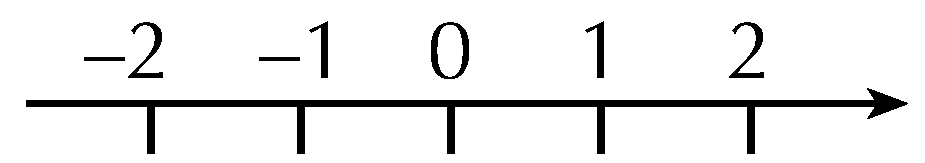
\includegraphics[height=10mm]{pics/integers.pdf}
	\begin{block}{Die ganzen Zahlen}
		\begin{itemize}
			\item Die Zahlen
				\begin{align*}
				0,\pm1,\pm2,\pm3,\ldots
				\end{align*}
				nennen wir die {\em ganzen Zahlen}.
			\item Wir k\oe nnen die ganzen Zahlen auf der Zahlengeraden abtragen.
			\item Mit $\ZZ$ wird die Menge der ganzen Zahlen bezeichnet.
		\end{itemize}
	\end{block}
\end{frame}

\begin{frame}\frametitle{\mytitle}
	\hfill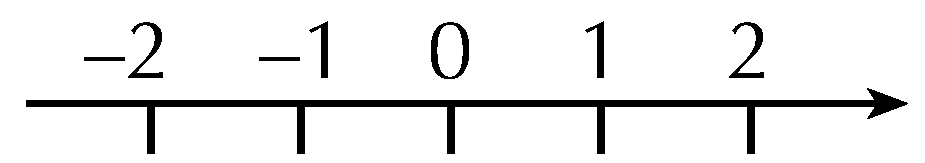
\includegraphics[height=10mm]{pics/integers.pdf}
	\begin{block}{Rechnen mit ganzen Zahlen}
		\begin{itemize}
			\item \emph{Addition:} man kann zwei ganze Zahlen addieren
			\item Beispiel:
				\begin{align*}
					1+1&=2&1+(-3)&=-2&-7+0&=-7
				\end{align*}
			\item Sie haben in der Schule ein Rechenschema kennengelernt, mit dem die Addition ausgef\ue hrt werden kann.
			\item Die Null verh\ae lt sich bei der Addition \emph{neutral}, d.h.\
				\begin{align*}
					0+x&=x\qquad\mbox{ f\ue r alle }x\in\ZZ
				\end{align*}
		\end{itemize}
	\end{block}
\end{frame}

\begin{frame}\frametitle{\mytitle}
	\hfill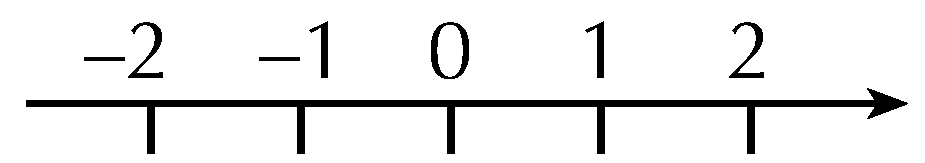
\includegraphics[height=10mm]{pics/integers.pdf}
	\begin{block}{Rechnen mit ganzen Zahlen}
		\begin{itemize}
			\item \emph{Negation:} zu jeder ganzen Zahl $x$ gibt es eine negative Zahl $-x$.
			\item Beispiel:
				\begin{align*}
					-7\mbox{ ist das Negative von }7\\
					7\mbox{ ist das Negative von }-7\\
					0\mbox{ ist das Negative von }0
				\end{align*}
			\item Es gilt die Rechenregel $-(-x)=x$.
			\item Das Negative hat die Eigenschaft
				\begin{align*}
					x+(-x)&=0.
				\end{align*}
		\end{itemize}
	\end{block}
\end{frame}

\begin{frame}\frametitle{\mytitle}
	\hfill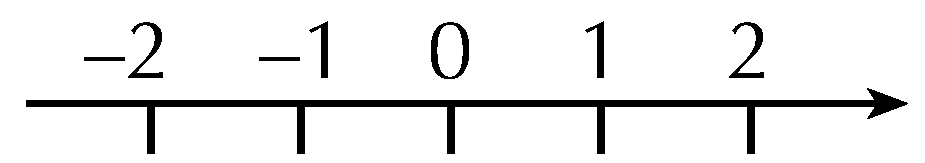
\includegraphics[height=10mm]{pics/integers.pdf}
	\begin{block}{Rechnen mit ganzen Zahlen}
		\begin{itemize}
			\item \emph{Multiplikation:} man kann zwei ganze Zahlen $x,y$ multiplizieren.
			\item Beispiel:
				\begin{align*}
					1\cdot 1&=1&0\cdot 5&=0&(-5)\cdot7&=-35
				\end{align*}
			\item Aus der Schule kennen Sie ein Rechenschma f\ue r die Multiplikation.
			\item Die Zahl $1$ verh\ae lt sich neutral bzgl.\ der Multiplikation:
				\begin{align*}
					1\cdot x&=x&&\mbox{f\ue r alle }x\in\ZZ
				\end{align*}
		\end{itemize}
	\end{block}
\end{frame}

\begin{frame}\frametitle{\mytitle}
	\hfill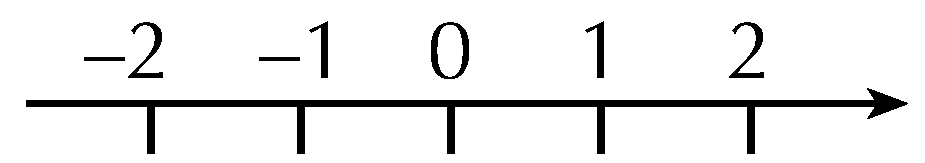
\includegraphics[height=10mm]{pics/integers.pdf}
	\begin{block}{Rechnen mit ganzen Zahlen}
		\begin{itemize}
			\item \emph{Distributivgesetz:} 
				die Addition und die Multiplikation sind miteinander verbunden durch die Regel
				\begin{align*}
					a\cdot(b+c)&=a\cdot b+a\cdot c&&\mbox{f\ue r alle }a,b,c\in\ZZ
				\end{align*}
			\item \alert{Beispiel:}
				\begin{align*}
					4\cdot2+4\cdot3=4\cdot(2+3)=4\cdot 5=20
				\end{align*}
		\end{itemize}
	\end{block}
\end{frame}

\begin{frame}\frametitle{\mytitle}
	\begin{block}{Rechenregeln f\ue r die ganzen Zahlen}
		F\ue r alle $x,y,z\in\ZZ$ gelten die folgenden Rechenregeln:
		\begin{description}
			\item[Kommutativgesetze:] 
					\begin{align*}
						x+y&=y+x,&x\cdot y&=y\cdot x
			\end{align*}
			\item[Assoziativgesetze:]	
				\begin{align*}
					(x+y)+z&=x+(y+z),&(x\cdot y)\cdot z&=x\cdot(y\cdot z)
				\end{align*}
			\item[Neutrales Element:]
				\begin{align*}
					0+x&=x,&1\cdot x&=x
				\end{align*}
			\item[Distributivgesetz:]
				\begin{align*}
					x\cdot(y+z)&=x\cdot y+x\cdot z
				\end{align*}
		\end{description}
	\end{block}
\end{frame}

\begin{frame}\frametitle{\mytitle}
	\begin{block}{Rechenregeln f\ue r die ganzen Zahlen}
		\begin{description}
			\item[Negation:] 
					\begin{align*}
						x+(-x)&=0
			\end{align*}
		\end{description}
	\end{block}
\end{frame}

\begin{frame}\frametitle{\mytitle}
	\begin{block}{Anordnung}
	\begin{itemize}
	\item Die ganzen Zahlen sind angeordnet, d.h.\ f\ue r alle $x\in\ZZ$ gilt genau eine der drei Aussagen:
		\begin{align*}
			x<0\mbox{ oder }x=0\mbox{ oder }x>0
		\end{align*}
	\item Die Anordnung erf\ue llt die Bedingungen:
		\begin{align*}
			x>0\mbox{ und }y>0\quad&\Rightarrow\quad x+y>0\\
			x>0\mbox{ und }y>0\quad&\Rightarrow\quad x\cdot y>0
		\end{align*}
	\end{itemize}
	\end{block}
\end{frame}

\begin{frame}\frametitle{\mytitle}
	\begin{block}{Die Division}
	\begin{itemize}
		\item Zu jeder Zahl $x\in\ZZ$ hat die Zahl $-x$ die Eigenschaft
			\begin{align*}
				x+(-x)&=0
			\end{align*}
		\item Es gibt aber im allgemeinen keine inversen Elemente bez\ue glich der Multiplikation.
		\item Beispielsweise gibt es keine Zahl $y\in\ZZ$, so da\ss\
			\begin{align*}
			2\cdot y=1
			\end{align*}
		\item Deshalb f\ue hrt man die rationalen Zahlen ein.
	\end{itemize}
	\end{block}
\end{frame}

\begin{frame}\frametitle{\mytitle}
	\begin{block}{Rationale Zahlen}
	\begin{itemize}
		\item Die Br\ue che der Form
			\begin{align*}
			\frac{x}{y}
			\end{align*}
			mit $x,y\in\ZZ$ und $y\neq0$ hei\ss en die \emph{rationalen Zahlen}.
		\item \alert{Beispiele:}
			\begin{align*}
				\frac{1}{2}\qquad\frac{-3}{4}\qquad\frac{9}{1}&\qquad\frac{0}{-7}
			\end{align*}
		\item Mit $\QQ$ wird die Menge aller rationalen Zahlen bezeichnet.
		\item $\QQ$ enth\ae lt $\ZZ$ als Teilmenge, weil jede ganze Zahl $z$ als Bruch $\frac{z}{1}$ geschrieben werden kann.
	\end{itemize}
	\end{block}
\end{frame}

\begin{frame}\frametitle{\mytitle}
	\begin{block}{Rationale Zahlen}
	\begin{itemize}
		\item Anders als ganze Zahlen haben rationale Zahlen mehrdeutige Darstellungen.
		\item \alert{Beispiel:}
			\begin{align*}
				\frac{1}{2}&=\frac{2}{4}=\frac{3}{6}=\frac{-1}{-2}=\frac{-8}{-16}
			\end{align*}
		\item Zwei Br\ue che $\frac{a}{b}$ und $\frac{c}{d}$ sind genau dann gleich, wenn
			\begin{align*}
			a\cdot d=b\cdot c
			\end{align*}
	\end{itemize}
	\end{block}
\end{frame}

\begin{frame}\frametitle{\mytitle}
	\begin{block}{Rationale Zahlen}
	\begin{itemize}
		\item Sie haben in der Schule gelernt, wie man mit rationalen Zahlen rechnet.
		\item \alert{Addition:}
			\begin{align*}
				\frac{a}{b}+\frac{c}{d}&=\frac{a\cdot d+b\cdot c}{b\cdot d}
			\end{align*}
		\item \alert{Multiplikation:}
			\begin{align*}
				\frac{a}{b}\cdot\frac{c}{d}&=\frac{a\cdot c}{b\cdot d}
			\end{align*}
		\item \alert{Beispiel:}
			\begin{align*}
				\frac{3}{2}+\frac{-1}{3}&=\frac{3\cdot 3+(-1)\cdot 2}{2\cdot 3}=\frac{7}{6}\\
				\frac{3}{2}\cdot\frac{-1}{3}&=\frac{3\cdot(-1)}{2\cdot 3}=\frac{-3}{6}=\frac{-1}{2}
			\end{align*}
	\end{itemize}
	\end{block}
\end{frame}

\begin{frame}\frametitle{\mytitle}
	\begin{block}{Rechenregeln f\ue r die rationalen Zahlen}
		F\ue r alle $x,y,z\in\QQ$ gelten die folgenden Rechenregeln:
		\begin{description}
			\item[Kommutativgesetze:] 
					\begin{align*}
						x+y&=y+x,&x\cdot y&=y\cdot x
			\end{align*}
			\item[Assoziativgesetze:]	
				\begin{align*}
					(x+y)+z&=x+(y+z),&(x\cdot y)\cdot z&=x\cdot(y\cdot z)
				\end{align*}
			\item[Neutrales Element:]
				\begin{align*}
					0+x&=x,&1\cdot x&=x
				\end{align*}
			\item[Distributivgesetz:]
				\begin{align*}
					x\cdot(y+z)&=x\cdot y+x\cdot z
				\end{align*}
		\end{description}
	\end{block}
\end{frame}

\begin{frame}\frametitle{\mytitle}
	\begin{block}{Rechenregeln f\ue r die rationalen Zahlen}
		\begin{description}
			\item[Negation:] jede rationale Zahl $x$ hat eine negative Zahl $-x$ mit
					\begin{align*}
						x+(-x)&=0
					\end{align*}
			\item[Inverses Element:]	
				zu jeder Zahl $x=\frac{a}{b}\in\QQ\setminus\cbc 0$ gibt es ein inverses Element $x^{-1}=\frac{b}{a}\in\QQ$, so da\ss\
				\begin{align*}
					x\cdot x^{-1}&=1
				\end{align*}
		\end{description}
		\alert{Beispiel:} $\bc{\frac{3}{4}}^{-1}=\frac{4}{3}$ und $\frac{3}{4}\cdot\frac{4}{3}=\frac{12}{12}=1$
	\end{block}
\end{frame}

\begin{frame}\frametitle{\mytitle}
	\begin{block}{Anordnung}
	\begin{itemize}
	\item Die rationalen Zahlen sind angeordnet, d.h.\ f\ue r alle $x\in\QQ$ gilt genau eine der drei Aussagen:
		\begin{align*}
			x<0\mbox{ oder }x=0\mbox{ oder }x>0
		\end{align*}
	\item Die Anordnung erf\ue llt die Bedingungen:
		\begin{align*}
			x>0\mbox{ und }y>0\quad&\Rightarrow\quad x+y>0\\
			x>0\mbox{ und }y>0\quad&\Rightarrow\quad x\cdot y>0
		\end{align*}
	\end{itemize}
	\end{block}
\end{frame}

\begin{frame}\frametitle{\mytitle}
	\begin{block}{Dezimalzahlen}
	\begin{itemize}
		\item Einige rationale Zahlen haben eine Darstellung als endliche ``Kommazahlen''.
		\item \alert{Beispiele:}
			\begin{align*}
				\frac{1}{2}=0.5\qquad\frac{2}{1}=2\qquad\frac{-9}{8}&=-1.125
			\end{align*}
		\item Sie erinnern aus der Schule, wie man mit endlichen Dezimalzahlen rechnet.
		\item (Wir werden es auch in den \Ue bungen wiederholen.)
		\item Allerdings besitzen nicht alle rationalen Zahlen so eine endliche Dezimaldarstellung.
		\item \alert{Beispiel:}
			\begin{align*}
				\frac{1}{9}=0.1111\cdots&=0.\overline 1
			\end{align*}
	\end{itemize}
	\end{block}
\end{frame}

\begin{frame}\frametitle{\mytitle}
	\begin{block}{Die reellen Zahlen}
	\begin{itemize}
		\item Eine \emph{reelle Zahl} ist eine Zahl, die eine unendliche Dezimaldarstellung
			\begin{align*}
			\pm p_\ell\cdots p_1.q_1q_2q_3\cdots
			\end{align*}
			mit $p_i,q_i\in\{0,1,2,3,4,5,6,7,8,9\}$ besitzt.
		\item Mit $\RR$ wird die Menge der reellen Zahlen bezeichnet.
	\end{itemize}
	\end{block}
\end{frame}

\begin{frame}\frametitle{\mytitle}
	\begin{block}{Beispiele}
	\begin{itemize}
		\item Jede ganze Zahl ist eine reelle Zahl:
			\begin{align*}
				-5&=-5.00000\cdots
			\end{align*}
		\item Jede endliche Dezimalzahl ist eine reelle Zahl:
			\begin{align*}
				0.12345&=0.1234500000\cdots
			\end{align*}
		\item Jede rationale Zahl ist eine reelle Zahl:
			\begin{align*}
				\frac{1}{9}&=0.1111111\cdots
			\end{align*}
	\end{itemize}
	\end{block}
\end{frame}

\begin{frame}\frametitle{\mytitle}
	\begin{block}{Beispiele}
	\begin{itemize}
		\item Es gibt aber auch reelle Zahlen, die keine rationalen Zahlen sind.
		\item Die Quadratwurzel aus 2:
			\begin{align*}
				\sqrt 2&=1.4142135623730950488016887242\cdots
			\end{align*}
		\item Die Kreiszahl $\pi$:
			\begin{align*}
				\pi&=3.1415926535897932384626433833\cdots
			\end{align*}
	\end{itemize}
	\end{block}
\end{frame}

\begin{frame}\frametitle{\mytitle}
	\begin{block}{Rechnen mit reellen Zahlen}
	\begin{itemize}
		\item Weil reelle Zahlen wom\oe glich keine endliche Darstellung besitzen, k\oe nnen wir mit ihnen nicht unmittelbar rechnen.
		\item Wir k\oe nnen zwar mit endlichen Ann\ae herungen rechnen.
		\item Aber es ist nicht ganz einfach, die Rechenoperationen wir $+$ und $\,\cdot\,$ direkt f\ue r reelle Zahlen zu definieren.
	\end{itemize}
	\end{block}
\end{frame}

\begin{frame}\frametitle{\mytitle}
	\hfill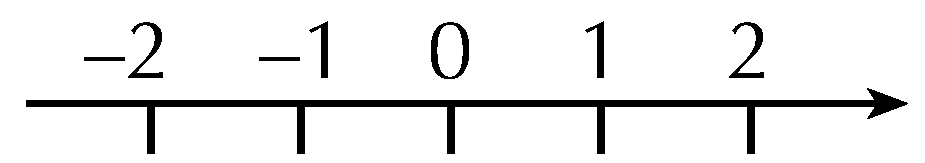
\includegraphics[height=10mm]{pics/integers.pdf}
	\begin{block}{Geometrische Interpretation}
	\begin{itemize}
		\item wir k\oe nnen uns die reellen Zahlen als Punkte auf der Zahlengeraden vorstellen.
		\item zumindest die Rechenoperationen $+$ und $-$ k\oe nnen wir uns dann geometrisch vorstellen.
	\end{itemize}
	\end{block}
\end{frame}

\begin{frame}\frametitle{\mytitle}
	\hfill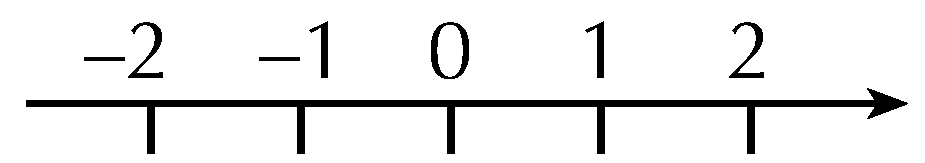
\includegraphics[height=10mm]{pics/integers.pdf}
	\begin{block}{Der axiomatische Ansatz}
	\begin{itemize}
		\item da wir die Rechenoperationen $+$ und $\,\cdot\,$ nicht direkt definieren k\oe nnen, werden wir stattdessen \emph{postulieren}, da\ss\ es eine sinnvolle Definition dieser Operationen gibt.
		\item `sinnvoll' bedeutet dabei, dass sich die Rechengesetze der rationalen Zahlen auf die reellen Zahlen verallgemeinern.
		\item au\ss erdem werden wir mit dem \alert{Vollst\ae ndigkeitsaxiom} postulieren, dass die reellen Zahlen die Zahlengerade ganz ausf\ue llen.
	\end{itemize}
	\end{block}
\end{frame}

\begin{frame}\frametitle{\mytitle}
	\begin{block}{Axiome f\ue r die reellen Zahlen}
		F\ue r alle $x,y,z\in\RR$ gelten die folgenden Rechenregeln:
\begin{description}
			\item[Kommutativgesetze:] 
					\begin{align*}
						x+y&=y+x,&x\cdot y&=y\cdot x
			\end{align*}
			\item[Assoziativgesetze:]	
				\begin{align*}
					(x+y)+z&=x+(y+z),&(x\cdot y)\cdot z&=x\cdot(y\cdot z)
				\end{align*}
			\item[Neutrales Element:]
				\begin{align*}
					0+x&=x,&1\cdot x&=x
				\end{align*}
			\item[Distributivgesetz:]
				\begin{align*}
					x\cdot(y+z)&=x\cdot y+x\cdot z
				\end{align*}
		\end{description}
	\end{block}
\end{frame}

\begin{frame}\frametitle{\mytitle}
	\begin{block}{Axiome f\ue r die reellen Zahlen}
		\begin{description}
			\item[Negation:] jede reelle Zahl $x$ hat eine negative Zahl $-x$ mit
					\begin{align*}
						x+(-x)&=0
					\end{align*}
			\item[Inverses Element:]	
				zu jeder reellen Zahl $x\neq0$ gibt es ein inverses Element $x^{-1}$, so da\ss\
				\begin{align*}
					x\cdot x^{-1}&=1
				\end{align*}
		\end{description}
	\end{block}
\end{frame}

\begin{frame}\frametitle{\mytitle}
	\begin{block}{Anordnungsaxiome}
	\begin{itemize}
	\item Die reellen Zahlen sind angeordnet, d.h.\ f\ue r alle $x\in\RR$ gilt genau eine der drei Aussagen:
		\begin{align*}
			x<0\mbox{ oder }x=0\mbox{ oder }x>0
		\end{align*}
	\item Die Anordnung erf\ue llt die Bedingungen:
		\begin{align*}
			x>0\mbox{ und }y>0\quad&\Rightarrow\quad x+y>0\\
			x>0\mbox{ und }y>0\quad&\Rightarrow\quad x\cdot y>0
		\end{align*}
	\end{itemize}
	\end{block}
\end{frame}

\begin{frame}\frametitle{\mytitle}
	\begin{block}{Obere Schranken}
	\begin{itemize}
		\item Sei $S\subseteq\RR$ eine Menge reeller Zahlen.
		\item Eine Zahl $u\in\RR$ hei\ss t \emph{obere Schranke} von $S$, falls
			\begin{align*}
				s\leq u\qquad\mbox{f\ue r alle }s\in S.
			\end{align*}
		\item Die Menge $S$ hei\ss t \emph{nach oben beschr\ae nkt}, wenn es eine obere Schranke $u$ gibt.
		\item Eine obere Schranke $u\in\RR$ hei\ss t \emph{Supremum} von $S$, falls f\ue r jede obere Schranke $v$ von $S$ gilt $u\leq v$.
		\item Mit anderen Worten: $u$ ist die \alert{kleinste} obere Schranke von $S$.
	\end{itemize}
	\end{block}
\end{frame}

\begin{frame}\frametitle{\mytitle}
	\begin{block}{Das Vollst\ae ndigkeitsaxiom}
	Jede nach oben beschr\ae nkte nichtleere Menge $\emptyset\neq S\subseteq\RR$ besitzt ein Supremum $\sup S$.
	\end{block}
\end{frame}

\begin{frame}\frametitle{\mytitle}
	\begin{block}{Untere Schranken}
	\begin{itemize}
		\item Sei $S\subseteq\RR$ eine Menge reeller Zahlen.
		\item Eine Zahl $u\in\RR$ hei\ss t \emph{untere Schranke} von $S$, falls
			\begin{align*}
				s\geq u\qquad\mbox{f\ue r alle }s\in S.
			\end{align*}
		\item Die Menge $S$ hei\ss t \emph{nach unten beschr\ae nkt}, wenn es eine untere Schranke $u$ gibt.
		\item Eine untere Schranke $u\in\RR$ hei\ss t \emph{Infimum} von $S$, falls f\ue r jede untere Schranke $v$ von $S$ gilt $u\geq v$.
		\item Mit anderen Worten: $u$ ist die \alert{gr\oe\ss te} untere Schranke von $S$.
		\item Eine Menge, die nach oben und unten beschr\ae nkt ist, nennt man \emph{beschr\ae nkt}.
	\end{itemize}
	\end{block}
\end{frame}

\begin{frame}\frametitle{\mytitle}
	\begin{block}{Beispiel}
	\begin{itemize}
		\item Sei $S=\cbc{s\in\RR:s^2\leq2}$.
		\item Die Menge $S$ ist nach oben beschr\ae nkt, weil $s\leq2$ f\ue r alle $s\in S$.
		\item D.h.\ 2 ist eine obere Schranke von $S$.
		\item Nach dem Vollst\ae ndigkeitsaxiom gibt es also eine reelle Zahl
			\begin{align*}
			u=\sup S.
			\end{align*}
		\item Wir wissen, da\ss\ $1.4\leq u\leq 1.5$.
		\item {\itshape Wir behaupten, da\ss\ $u^2=2$.}
	\end{itemize}
	\end{block}
\end{frame}

\begin{frame}\frametitle{\mytitle}
	\begin{block}{Beispiel}
	\begin{itemize}
		\item \alert{Angenommen $u^2<2$.}
		\item Dann ist $\delta=2-u^2>0$.
		\item Folglich gilt
			\begin{align*}
				(u+0.1\cdot\delta)^2=u^2+0.2\cdot\delta u+0.01\delta^2<u^2+\delta=2.
			\end{align*}
		\item Also ist $u+0.1\delta\in S$ und somit $u$ keine obere Schranke von $S$.
		\item Das widerspricht $u=\sup S$.
	\end{itemize}
	\end{block}
\end{frame}

\begin{frame}\frametitle{\mytitle}
	\begin{block}{Beispiel}
	\begin{itemize}
		\item \alert{Angenommen $u^2>2$.}
		\item Dann ist $\delta=u^2-2>0$.
		\item Folglich gilt
			\begin{align*}
				(u-0.1\cdot\delta)^2=u^2-0.2\cdot\delta u+0.01\delta^2>u^2-\delta=2.
			\end{align*}
		\item Also ist $u-0.1\delta$ eine obere Schranke von $S$.
		\item Das widerspricht $u=\sup S$.
	\end{itemize}
	\end{block}
\end{frame}

\begin{frame}\frametitle{\mytitle}
	\begin{block}{Beispiel}
	\begin{itemize}
		\item Wir haben also die Annahmen $u^2>2$ und $u^2<2$ zum Widerspruch gef\ue hrt.
		\item Folglich gilt $u^2=2$.
		\item Damit ist gezeigt, da\ss\ $u=\sqrt 2\in\RR$.
		\item {\itshape Das Beispiel zeigt auch, da\ss\ das Vollst\ae ndigkeitsaxiom nicht f\ue r die rationalen Zahlen $\QQ$ gilt -- warum?}
	\end{itemize}
	\end{block}
\end{frame}

\begin{frame}\frametitle{\mytitle}
	\begin{block}{Zusammenfassung}
	\begin{itemize}
		\item Wir haben die Menge $\RR$ der reellen Zahlen kennengelernt.
		\item Diese enth\ae lt die Menge $\QQ$ der rationalen Zahlen als eine echte Teilmenge.
		\item Die reellen Zahlen sind durch folgende Axiome characterisiert:
		\begin{itemize}
		\item Kommutativ- und Assoziativgesetze f\ue r Addition und Multiplikation.
		\item Neutralit\ae t von $0$ f\ue r die Additon und von $1$ f\ue r die Multiplikation.
		\item Jede Zahl $x\in\RR$ besitzt eine Negation $-x$.
		\item Jede Zahl $x\in\RR\setminus\cbc0$ besitzt ein Inverses $x^{-1}$.
		\item Das Distributivgesetz.
		\item Die Anordnungsaxiome.
		\item Das Vollst\ae ndigkeitsaxiom.
		\end{itemize}
	\end{itemize}
	\end{block}
\end{frame}
\end{document}
